
\documentclass[12pt]{article}
\usepackage[spanish]{babel}
\usepackage[utf8]{inputenc}
\usepackage{geometry}
\usepackage{graphicx}
\usepackage{booktabs}
\usepackage{array}
\usepackage{longtable}
\usepackage{setspace}
\usepackage{hyperref}
\usepackage{float}
\usepackage{caption}

\geometry{margin=2.5cm}
\singlespacing

\title{\textbf{Análisis de Indicadores Socioeconómicos\\del Departamento de Ica, 2014--2023}}
\author{Karen Medrano Valenzuela}
\date{\today}

\begin{document}
\maketitle
\tableofcontents
\newpage

%---------------------------------------
\section{Introducción}
%---------------------------------------
El departamento de Ica, ubicado en la costa sur del Perú, es una de las
regiones con mayor dinamismo económico del país. Su economía se sustenta
principalmente en la agricultura de exportación, la minería, la pesca y,
en menor medida, la manufactura y la construcción. En los últimos años,
Ica ha consolidado su posición como uno de los principales productores de
uva, espárrago y palta a nivel nacional, al tiempo que ha experimentado
un crecimiento notable en su sector minero, particularmente en la
producción de cobre.

El presente informe tiene como objetivo describir y analizar la evolución
de ocho sectores económicos y sociales del departamento de Ica durante
el período 2014--2023, utilizando datos oficiales del Instituto Nacional
de Estadística e Informática (INEI) y del Ministerio de Energía y Minas
(MINEM). Los sectores analizados comprenden: Participación Ciudadana,
Tecnologías de Información y Comunicación (TIC), Agrario, Pesca,
Minería e Hidrocarburos, Manufactura, Electricidad y Agua, y Construcción.

%---------------------------------------
\section{Sector 10: Participación Ciudadana}
%---------------------------------------
\subsection{Descripción del indicador}
La participación ciudadana en términos de documentación de identidad
constituye un indicador clave para medir la inclusión social y el acceso
a derechos fundamentales. El indicador 10.1 recoge el porcentaje de
población de 18 años a más que cuenta con Documento Nacional de Identidad
(DNI), desagregado por departamento, para el período 2014--2023.

\subsection{Análisis descriptivo}

\begin{table}[H]
\centering
\caption{Población de 18+ años con DNI - Ica, 2014-2023 (\%)}
\small
\begin{tabular}{lr}
\toprule
\textbf{Año} & \textbf{Ica (\%)} \\
\midrule
2,014.00 & 99.79 \\
2,015.00 & 99.54 \\
2,016.00 & 99.92 \\
2,017.00 & 99.87 \\
2,018.00 & 99.75 \\
2,019.00 & 99.75 \\
2,020.00 & 99.67 \\
2,021.00 & 98.57 \\
2,022.00 & 98.13 \\
2,023.00 & 99.67 \\
\bottomrule
\end{tabular}
\end{table}

La tabla anterior muestra que Ica ha mantenido niveles de documentación
consistentemente por encima del 98\% a lo largo del período estudiado,
lo que refleja un alto grado de formalización en términos de identidad
civil. Entre 2014 y 2019 los valores se mantuvieron relativamente
estables, con ligeras fluctuaciones por encima del 99\%.

\begin{figure}[H]
\centering
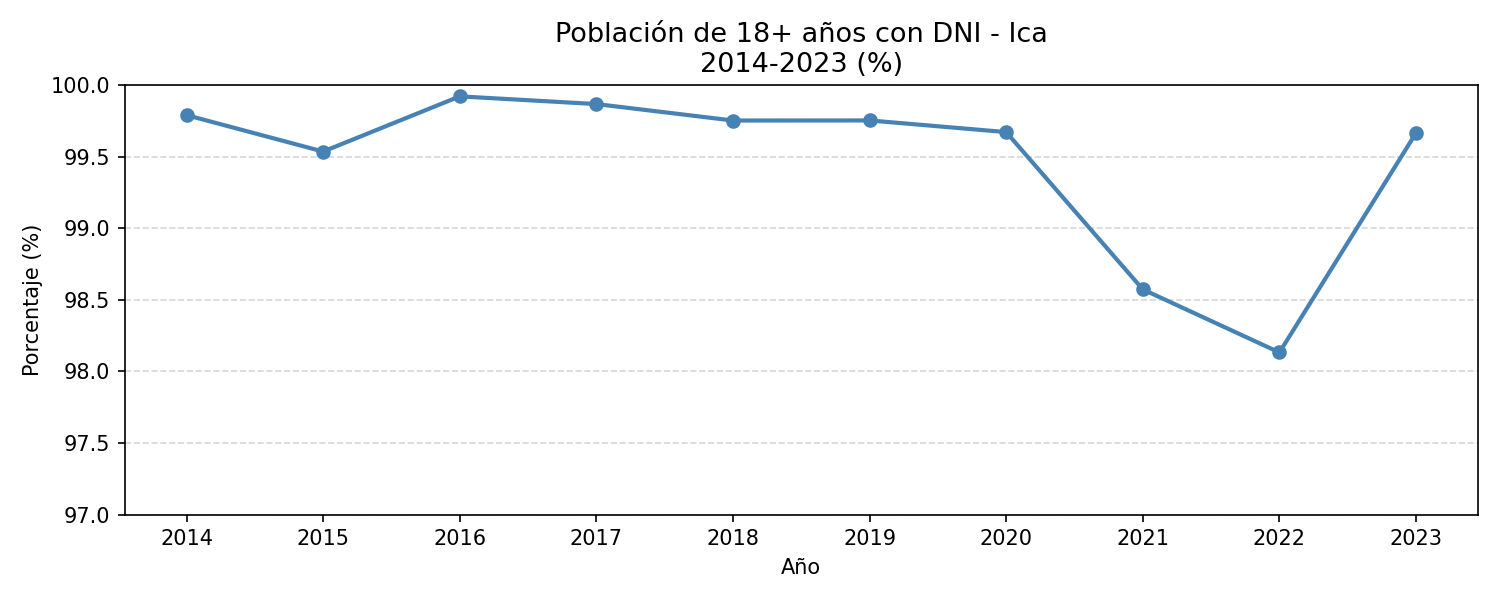
\includegraphics[width=0.9\textwidth]{grafico_10_1.png}
\caption{Evolución de la población con DNI -- Ica, 2014--2023 (\%)}
\end{figure}

\subsection{Interpretación}
El gráfico evidencia una tendencia estable con una caída perceptible
en los años 2021 y 2022, cuando el indicador bajó a 98.57\% y 98.13\%
respectivamente. Esta reducción coincide con el período de mayor impacto
de la pandemia por COVID-19, durante el cual las oficinas del RENIEC
operaron con restricciones de aforo y horario, dificultando la renovación
y obtención de documentos de identidad. Para 2023 el indicador se
recuperó hasta 99.67\%, retomando niveles similares a los previos a la
pandemia.

%---------------------------------------
\section{Sector 11: Tecnologías de Información y Comunicación}
%---------------------------------------
\subsection{Descripción del indicador}
Los indicadores TIC permiten medir el grado de acceso de los hogares
a distintos medios de comunicación y tecnología. Se analizan dos
subindicadores: el porcentaje de hogares con radio o equipo de sonido
(11.1) y el porcentaje de hogares con teléfono de línea fija (11.3),
ambos para Ica durante 2014--2023.

\subsection{Hogares con radio o equipo de sonido}

\begin{figure}[H]
\centering
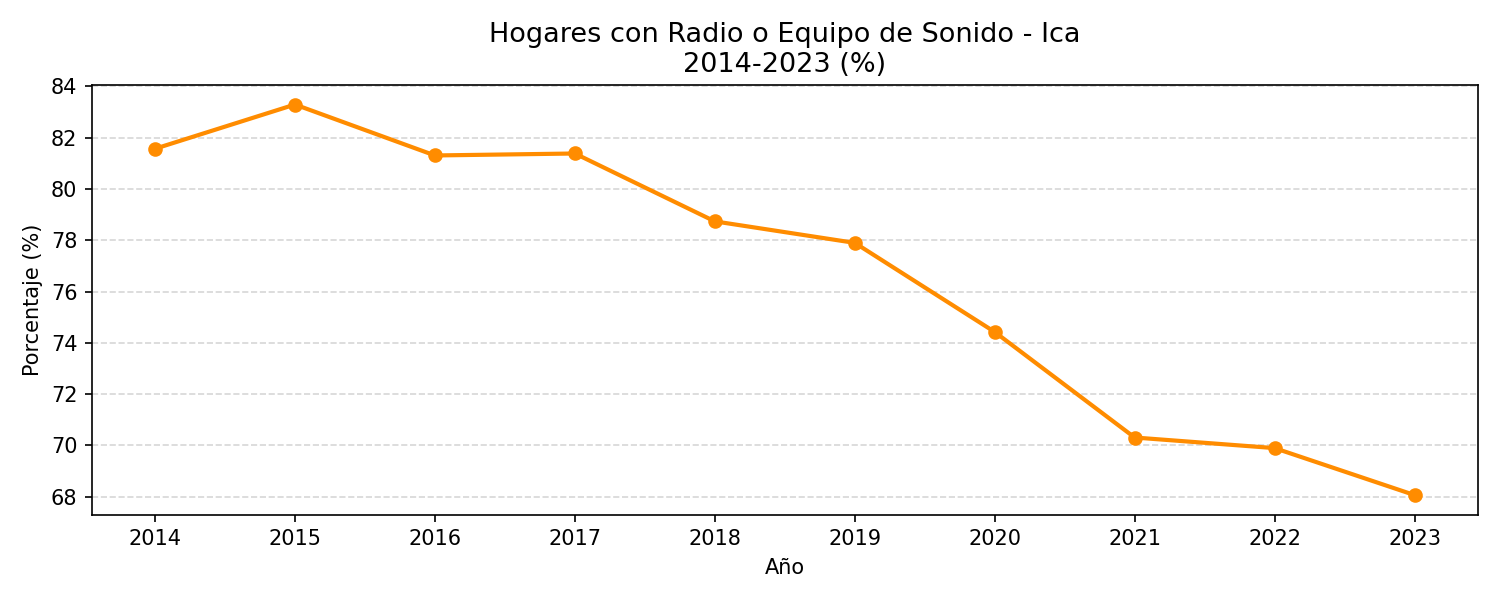
\includegraphics[width=0.9\textwidth]{grafico_11_1.png}
\caption{Hogares con radio o equipo de sonido -- Ica, 2014--2023 (\%)}
\end{figure}

El acceso a radio en los hogares iqueños muestra una tendencia
decreciente durante el período analizado. Si bien en 2014 el 81.6\%
de hogares contaba con este medio, hacia 2023 dicho porcentaje había
caído a 68.1\%. Esta reducción no necesariamente implica un retroceso
en el acceso a información, sino más bien una transición hacia nuevos
medios digitales como smartphones y plataformas de streaming, que
han ido desplazando a los equipos de radio tradicionales.

\subsection{Hogares con teléfono fijo}

\begin{table}[H]
\centering
\caption{Hogares con Teléfono Fijo - Ica, 2014-2023 (\%)}
\small
\begin{tabular}{lr}
\toprule
\textbf{Año} & \textbf{Ica (\%)} \\
\midrule
2,014.00 & 25.45 \\
2,015.00 & 23.12 \\
2,016.00 & 20.38 \\
2,017.00 & 21.16 \\
2,018.00 & 20.49 \\
2,019.00 & 17.64 \\
2,020.00 & 10.25 \\
2,021.00 & 7.18 \\
2,022.00 & 5.13 \\
2,023.00 & 4.86 \\
\bottomrule
\end{tabular}
\end{table}


\begin{figure}[H]
\centering
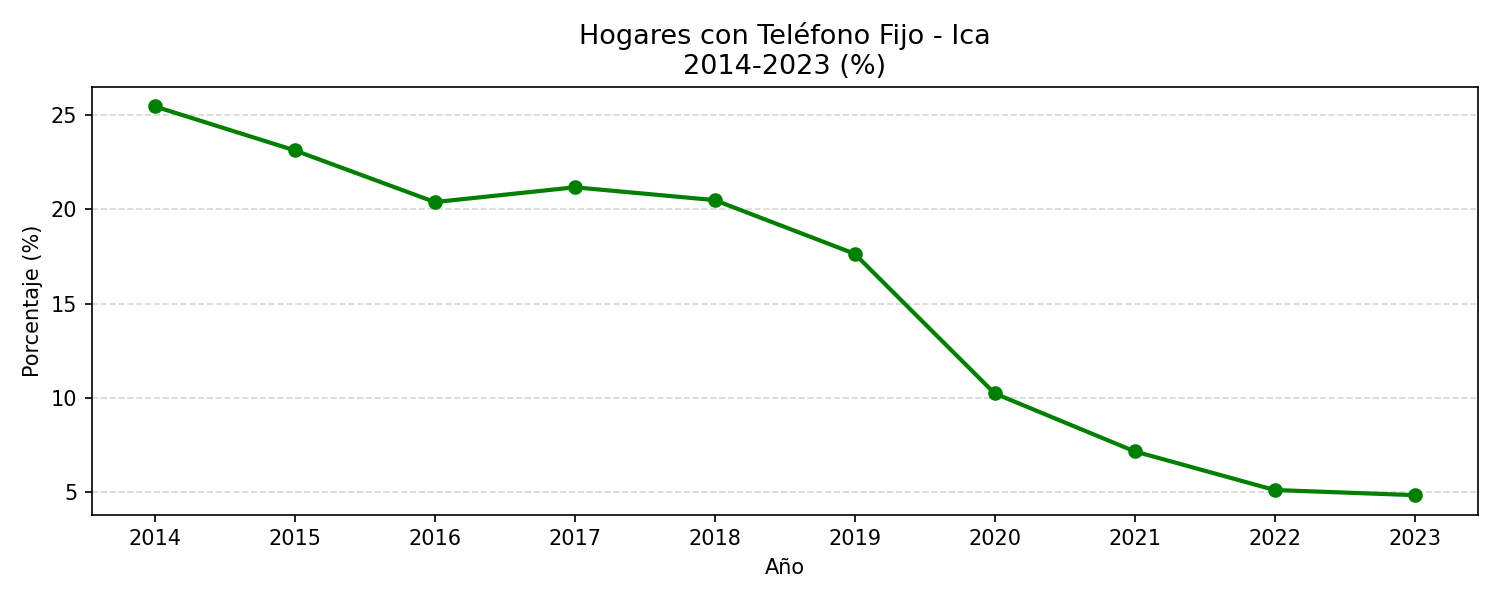
\includegraphics[width=0.9\textwidth]{grafico_11_3.png}
\caption{Hogares con teléfono fijo -- Ica, 2014--2023 (\%)}
\end{figure}

\subsection{Interpretación}
La caída del teléfono fijo en Ica es una de las tendencias más marcadas
del período. De representar el 25.45\% de los hogares en 2014, pasó
a apenas 4.86\% en 2023, una reducción de más de 20 puntos porcentuales
en solo nueve años. Este fenómeno responde al proceso de sustitución
tecnológica que se viene dando a nivel nacional e internacional, donde
la telefonía móvil ha reemplazado casi por completo a la línea fija,
especialmente en regiones de alta densidad urbana como Ica.

%---------------------------------------
\section{Sector 12: Agrario}
%---------------------------------------
\subsection{Descripción del indicador}
El sector agrario constituye uno de los pilares de la economía iqueña.
El indicador 12.2 registra la producción agropecuaria anual de Ica
según principales productos, expresada en toneladas métricas, para
el período 2015--2024.

\subsection{Análisis descriptivo}

\begin{table}[H]
\centering
\caption{Top 10 Productos Agropecuarios - Ica, años seleccionados (TM)}
\small
\begin{tabular}{lrrrr}
\toprule
\textbf{Producto} & \textbf{2015} & \textbf{2018} & \textbf{2021} & \textbf{2023} \\
\midrule
Uva  & 229,996.70 & 265,004.81 & 400,589.26 & 534,404.11 \\
Mandarina & 81,488.93 & 169,652.75 & 179,231.02 & 226,559.53 \\
Huevos & 132,270.82 & 193,850.80 & 224,771.24 & 217,796.98 \\
Maíz amarillo duro & 181,320.71 & 204,685.21 & 193,850.85 & 181,260.87 \\
Espárrago & 146,834.94 & 189,940.74 & 179,526.06 & 170,927.96 \\
Alfalfa & 162,848.98 & 132,486.53 & 146,440.99 & 167,402.14 \\
Papa (mejorada-nativa) & 98,037.43 & 118,485.63 & 119,440.32 & 136,089.60 \\
Ave & 78,416.66 & 92,193.04 & 110,876.44 & 122,924.42 \\
Tomate & 106,263.53 & 138,863.10 & 129,067.95 & 115,196.46 \\
Palta & 56,637.77 & 66,332.42 & 81,699.79 & 103,656.37 \\
\bottomrule
\end{tabular}
\end{table}


\begin{figure}[H]
\centering
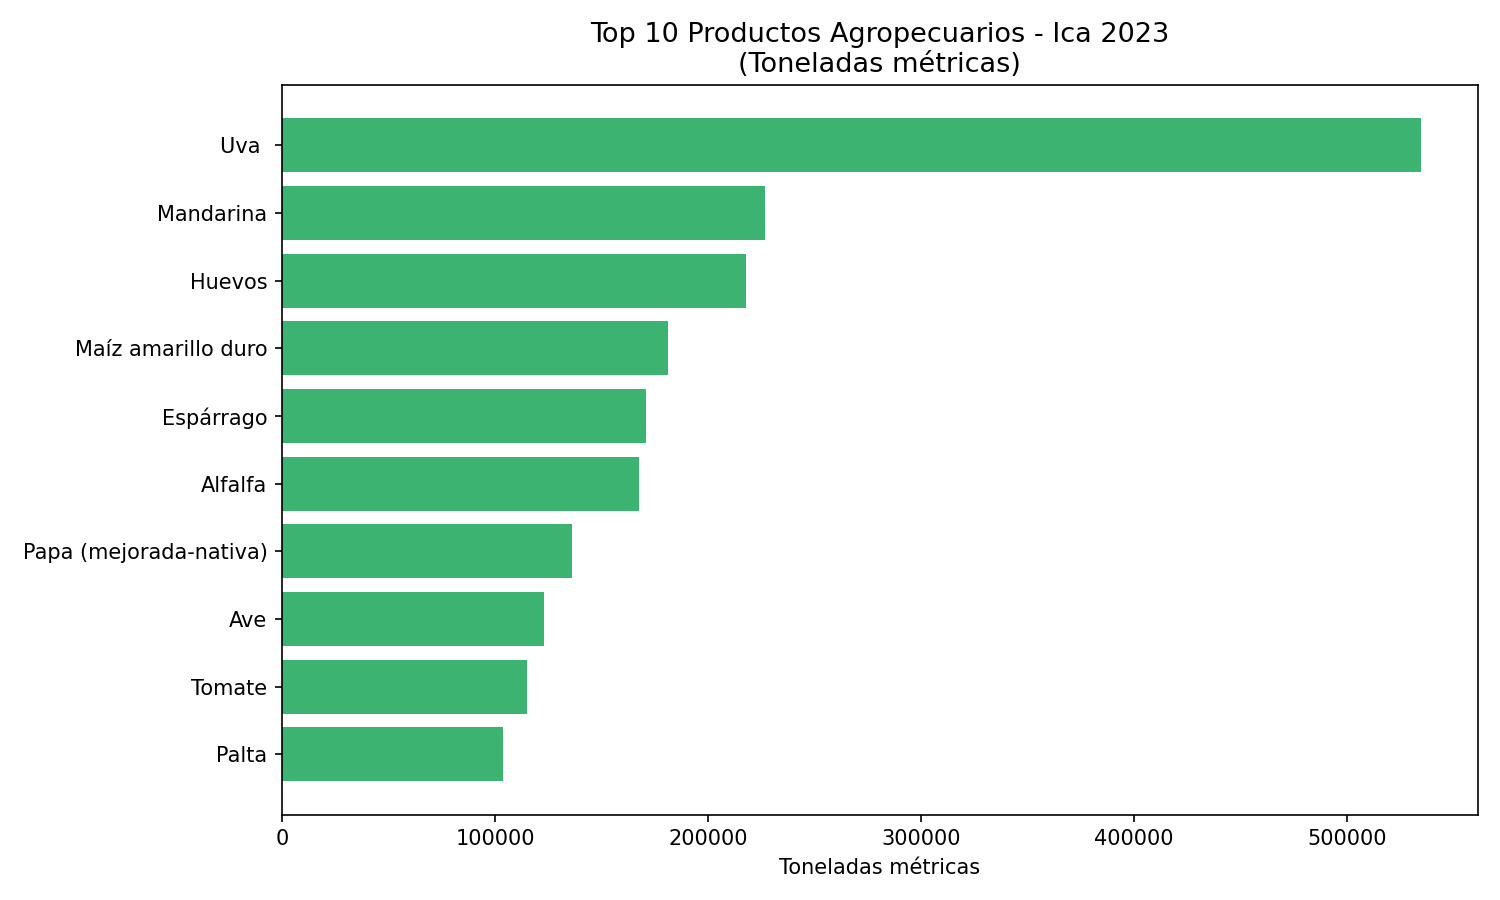
\includegraphics[width=0.9\textwidth]{grafico_12_2a.png}
\caption{Top 10 productos agropecuarios -- Ica, 2023 (TM)}
\end{figure}

\begin{figure}[H]
\centering
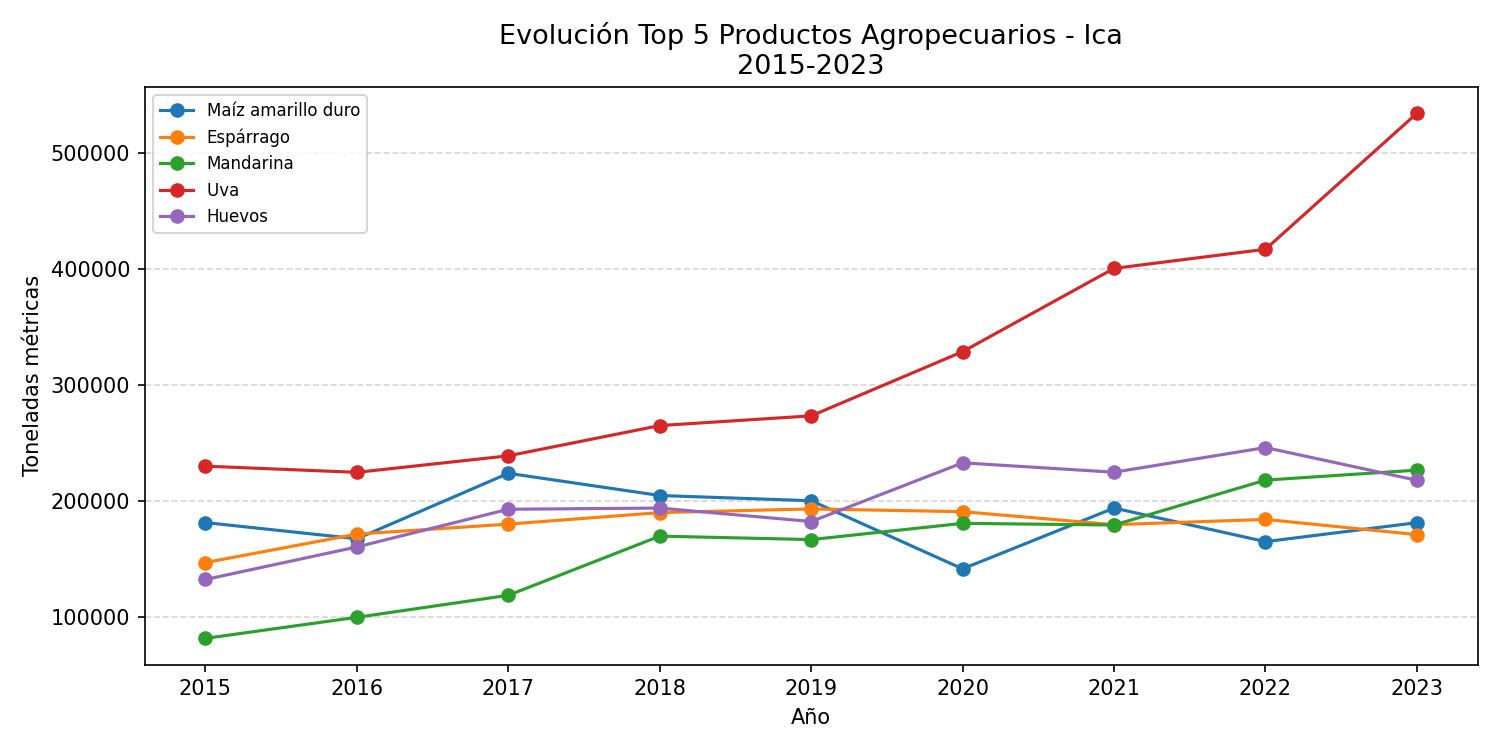
\includegraphics[width=0.9\textwidth]{grafico_12_2b.png}
\caption{Evolución top 5 productos agropecuarios -- Ica, 2015--2023}
\end{figure}

\begin{figure}[H]
\centering
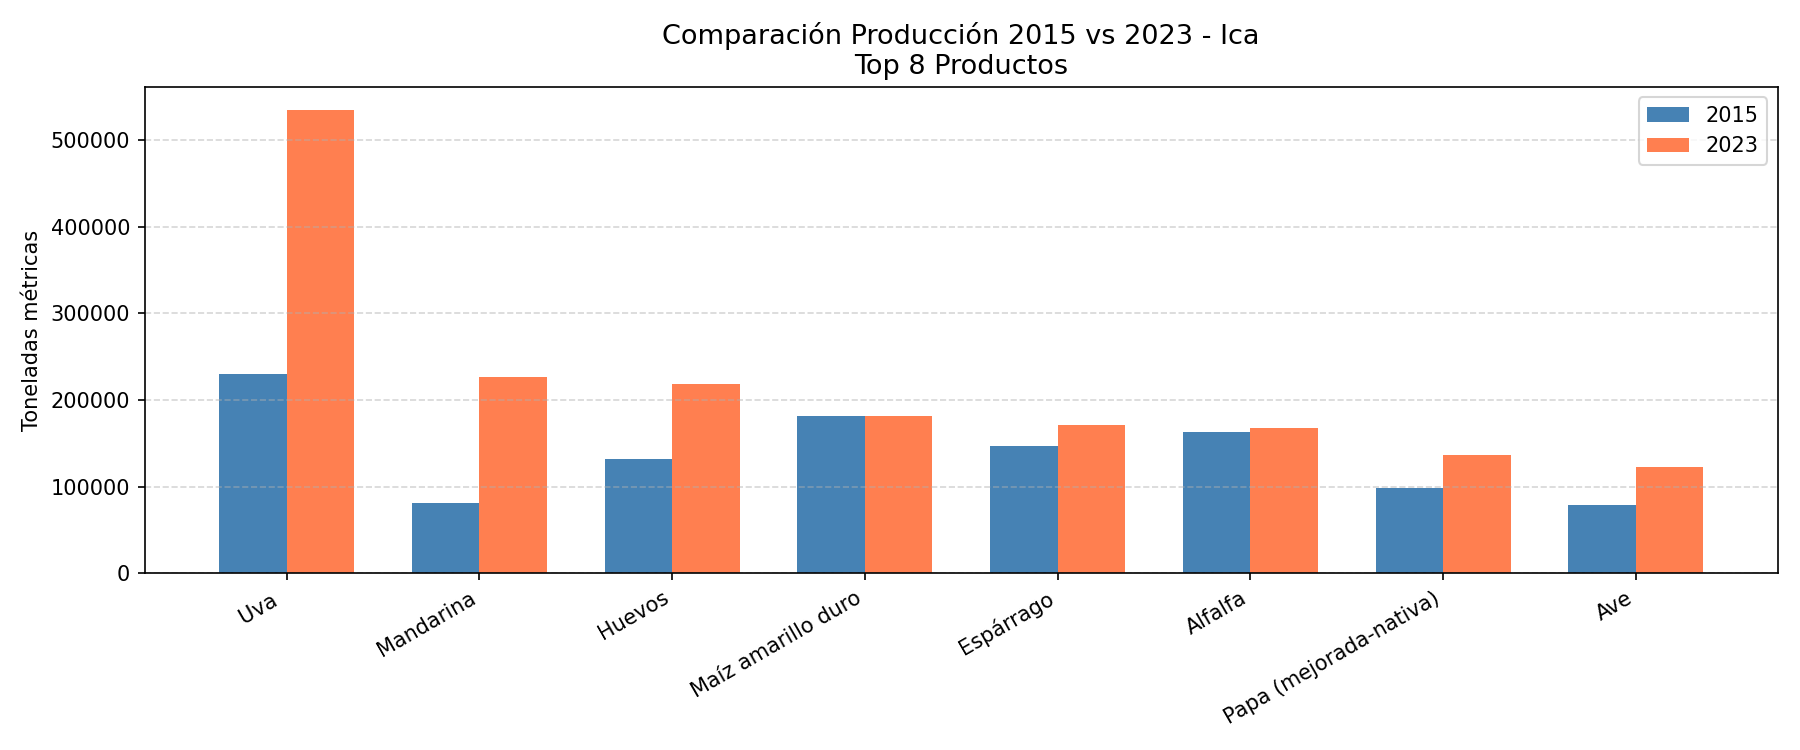
\includegraphics[width=0.9\textwidth]{grafico_12_2c.png}
\caption{Comparación producción 2015 vs 2023 -- Ica (TM)}
\end{figure}

\subsection{Interpretación}
La uva se consolida como el producto estrella de la agricultura iqueña,
con una producción que pasó de 229,997 TM en 2015 a 534,404 TM en 2023,
representando un incremento de más del 130\% en el período. Este
crecimiento responde a la creciente demanda internacional y a las
condiciones climáticas favorables del valle de Ica para su cultivo.

La mandarina también registró un crecimiento notable, triplicando su
producción entre 2015 y 2023. En contraste, productos como el algodón
tanguis y la cebolla mostraron caídas importantes, lo que refleja
cambios en la rentabilidad relativa de los cultivos y en las preferencias
del mercado exportador.

%---------------------------------------
\section{Sector 13: Pesca}
%---------------------------------------
\subsection{Descripción del indicador}
La pesca es una actividad productiva relevante en Ica dada su
ubicación costera. El indicador 13.2 registra el desembarque de
recursos marítimos para consumo humano directo, según puerto,
expresado en toneladas métricas brutas, para el período 2014--2023.

\subsection{Análisis descriptivo}

\begin{table}[H]
\centering
\caption{Desembarque Consumo Humano Directo - Ica, años seleccionados (TM)}
\small
\begin{tabular}{lrrrrrr}
\toprule
\textbf{Ámbito} & \textbf{2014} & \textbf{2016} & \textbf{2018} & \textbf{2020} & \textbf{2022} & \textbf{2023} \\
\midrule
Total País & 1,264,761.00 & 1,020,022.00 & 1,136,202.00 & 1,342,119.00 & 1,257,041.00 & 1,514,182.85 \\
Ica Total & 72,606.00 & 48,562.00 & 69,255.00 & 82,848.00 & 107,171.15 & 165,844.22 \\
Pisco & 10,676.00 & 24,855.00 & 18,394.00 & 20,263.00 & 63,333.10 & 84,815.67 \\
San Andrés & 38,501.00 & 13,540.00 & 34,033.00 & 19,714.00 & 21,319.95 & 29,400.80 \\
San Juan/San Nicolás & 7,921.00 & 9,872.00 & 15,983.00 & 20,572.00 & 5,432.00 & 15,569.56 \\
Tambo de Mora & 15,508.00 & 295.00 & 845.00 & 22,299.00 & 17,086.10 & 36,058.19 \\
\bottomrule
\end{tabular}
\end{table}


\begin{figure}[H]
\centering
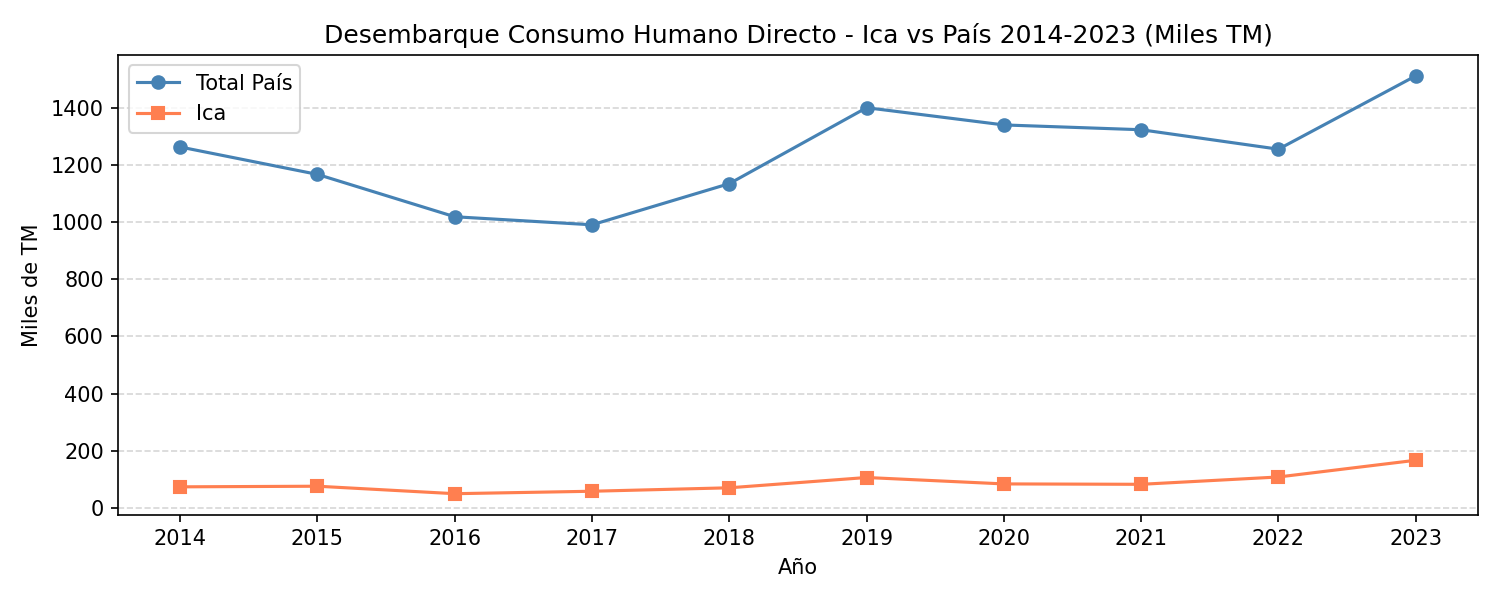
\includegraphics[width=0.9\textwidth]{grafico_13_1.png}
\caption{Desembarque consumo humano directo -- Ica vs País, 2014--2023 (Miles TM)}
\end{figure}

\begin{figure}[H]
\centering
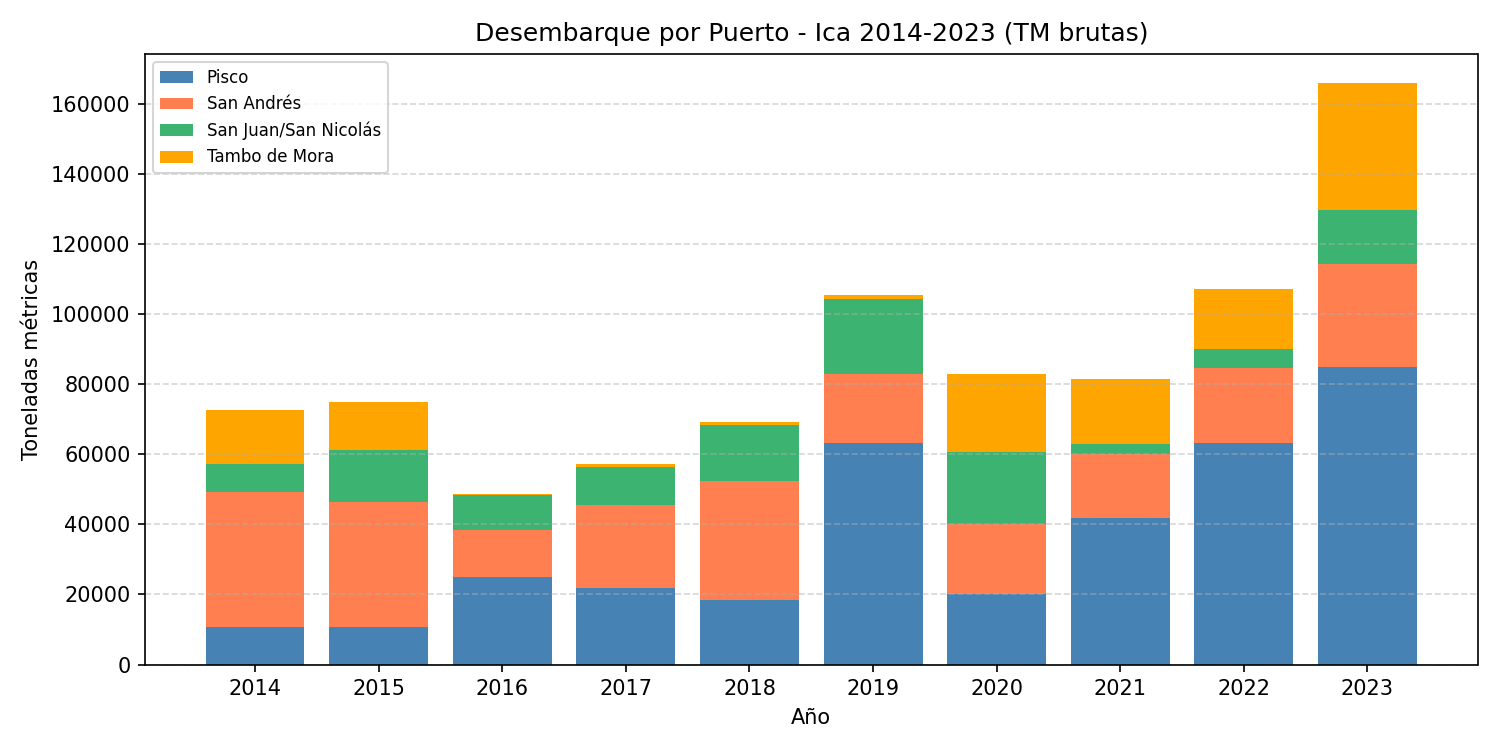
\includegraphics[width=0.9\textwidth]{grafico_13_2.png}
\caption{Desembarque por puerto -- Ica, 2014--2023 (TM brutas)}
\end{figure}

\subsection{Interpretación}
El desembarque pesquero en Ica muestra una recuperación sostenida
desde 2016, año en que registró su valor más bajo con 48,562 TM.
A partir de entonces la tendencia fue ascendente, llegando a 165,844 TM
en 2023, el valor más alto del período. El puerto de Pisco concentra
la mayor actividad, aunque San Andrés también tiene una participación
significativa. La caída de 2016 pudo estar relacionada con el fenómeno
de El Niño que afectó la biomasa disponible en esa temporada.

%---------------------------------------
\section{Sector 14: Minería e Hidrocarburos}
%---------------------------------------
\subsection{Descripción del indicador}
La minería metálica representa uno de los sectores con mayor
crecimiento en Ica durante la última década. Se analizan la producción
de minerales metálicos (14.1), la producción de cobre por departamento
(14.5), la producción de plata por departamento (14.6), el volumen
de exportación minera nacional (14.11) y el valor FOB de exportación
minera (14.12).

\subsection{Producción minera metálica en Ica}

\begin{table}[H]
\centering
\caption{Producción Minera Metálica - Ica, años seleccionados}
\small
\begin{tabular}{lrrrrr}
\toprule
\textbf{Producto} & \textbf{2016} & \textbf{2018} & \textbf{2020} & \textbf{2022} & \textbf{2023} \\
\midrule
Cobre & 43,155.23 & 59,899.50 & 40,869.22 & 192,137.00 & 216,349.46 \\
Plomo & 18,307.49 & 14,789.02 & 14,471.71 & 20,275.84 & 22,820.78 \\
Zinc & 181,054.15 & 138,435.20 & 132,473.31 & 116,946.11 & 142,009.28 \\
Plata & 134,530.37 & 123,196.66 & 98,944.99 & 223,295.79 & 219,199.29 \\
Oro & 248.18 & 199.58 & 288.36 & 522.91 & 532.80 \\
Hierro & 7,663,123.99 & 9,533,871.13 & 8,893,971.53 & 12,936,826.38 & 12,986,023.24 \\
\bottomrule
\end{tabular}
\end{table}


\begin{figure}[H]
\centering
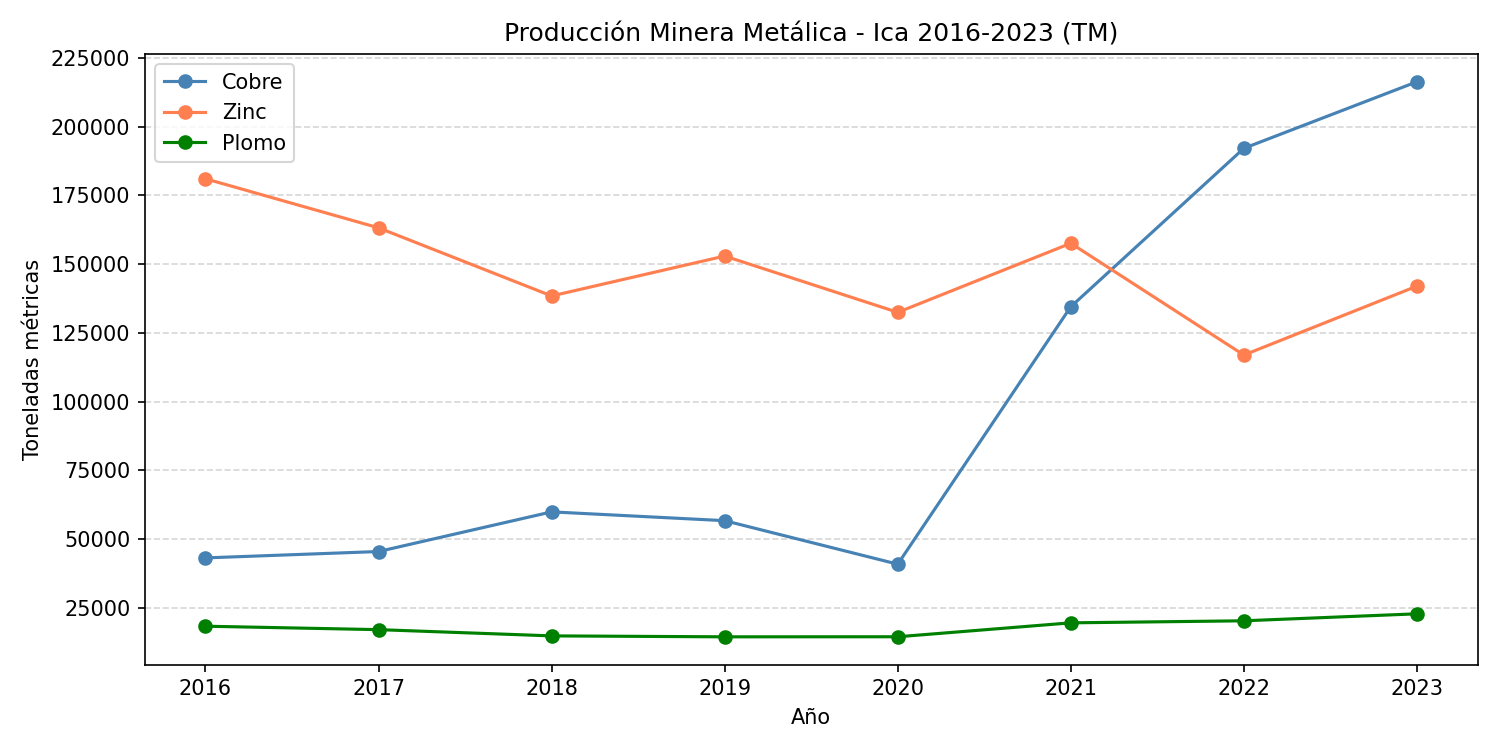
\includegraphics[width=0.9\textwidth]{grafico_14_1a.png}
\caption{Producción minera metálica -- Ica, 2016--2023 (TM)}
\end{figure}

\begin{figure}[H]
\centering
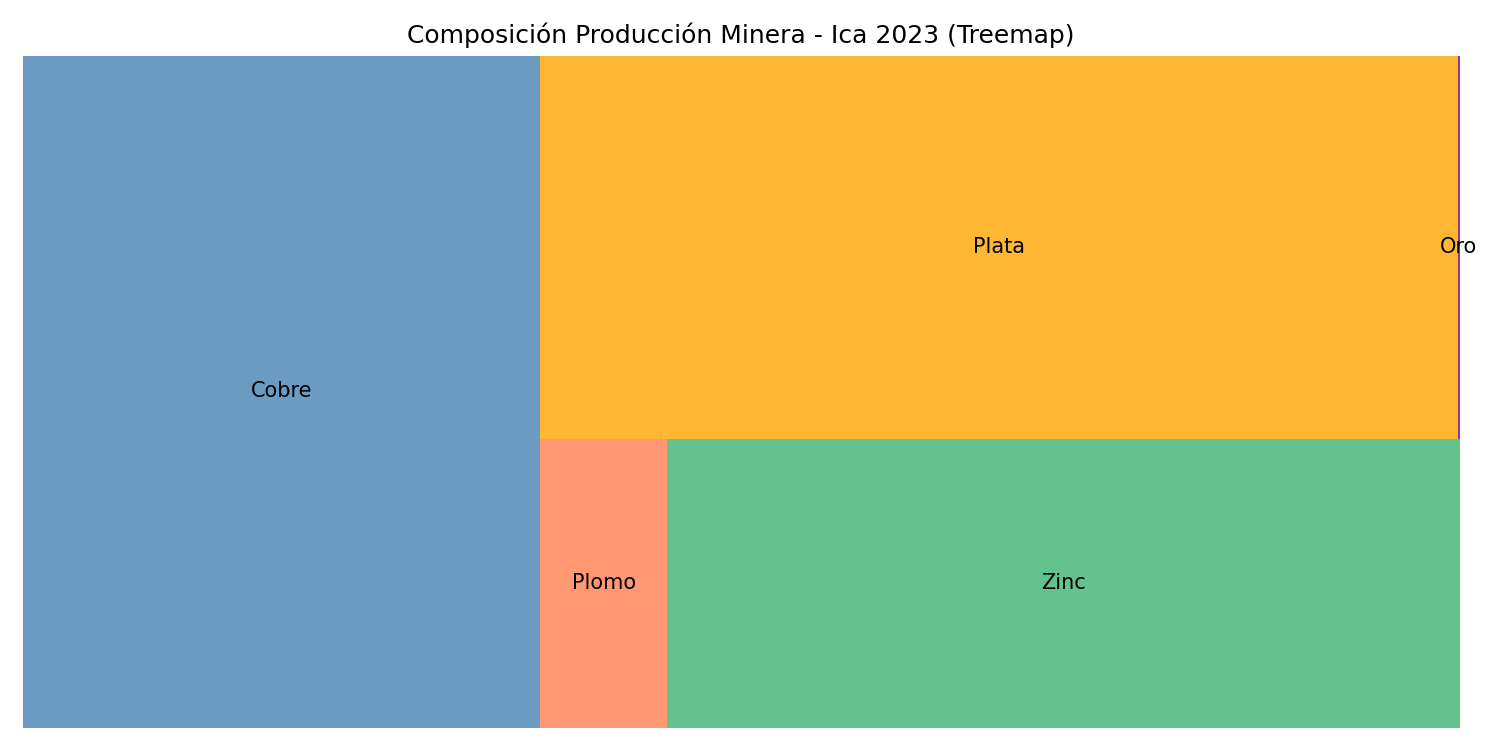
\includegraphics[width=0.9\textwidth]{grafico_14_1b.png}
\caption{Composición de la producción minera -- Ica, 2023 (Treemap)}
\end{figure}

\subsection{Producción de cobre}

\begin{figure}[H]
\centering
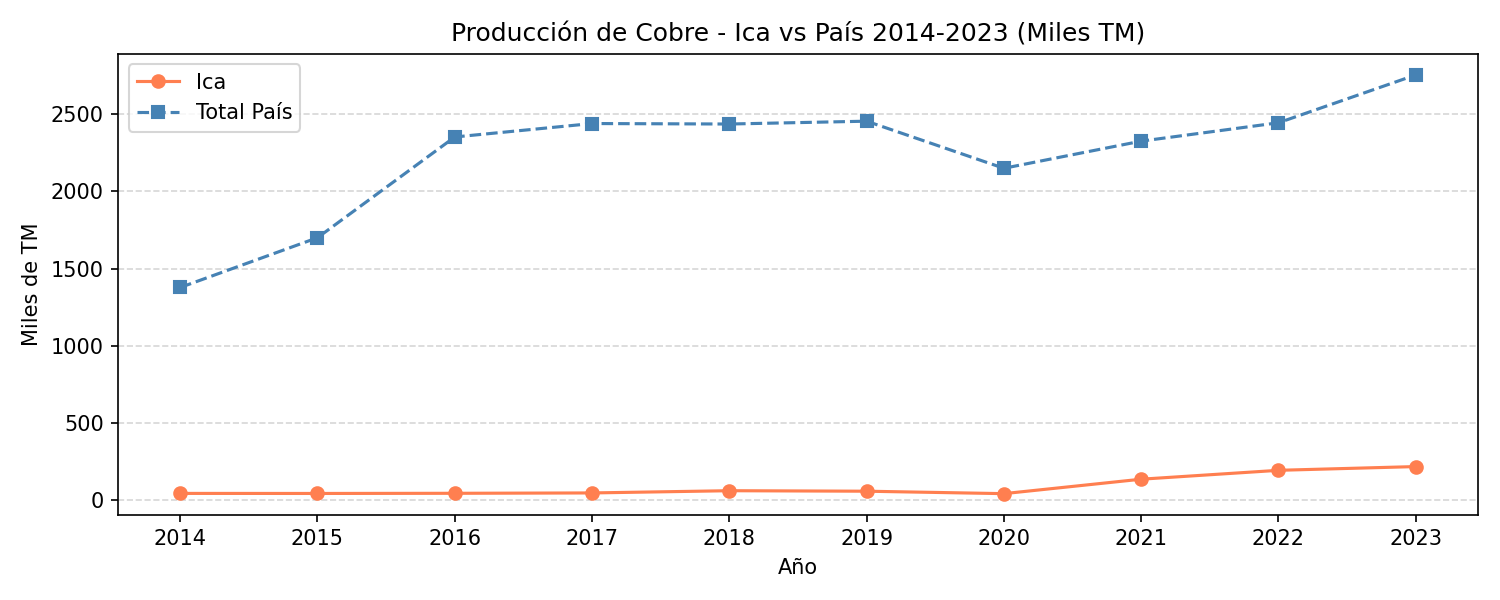
\includegraphics[width=0.9\textwidth]{grafico_14_5a.png}
\caption{Producción de cobre -- Ica vs País, 2014--2023 (Miles TM)}
\end{figure}

\begin{figure}[H]
\centering
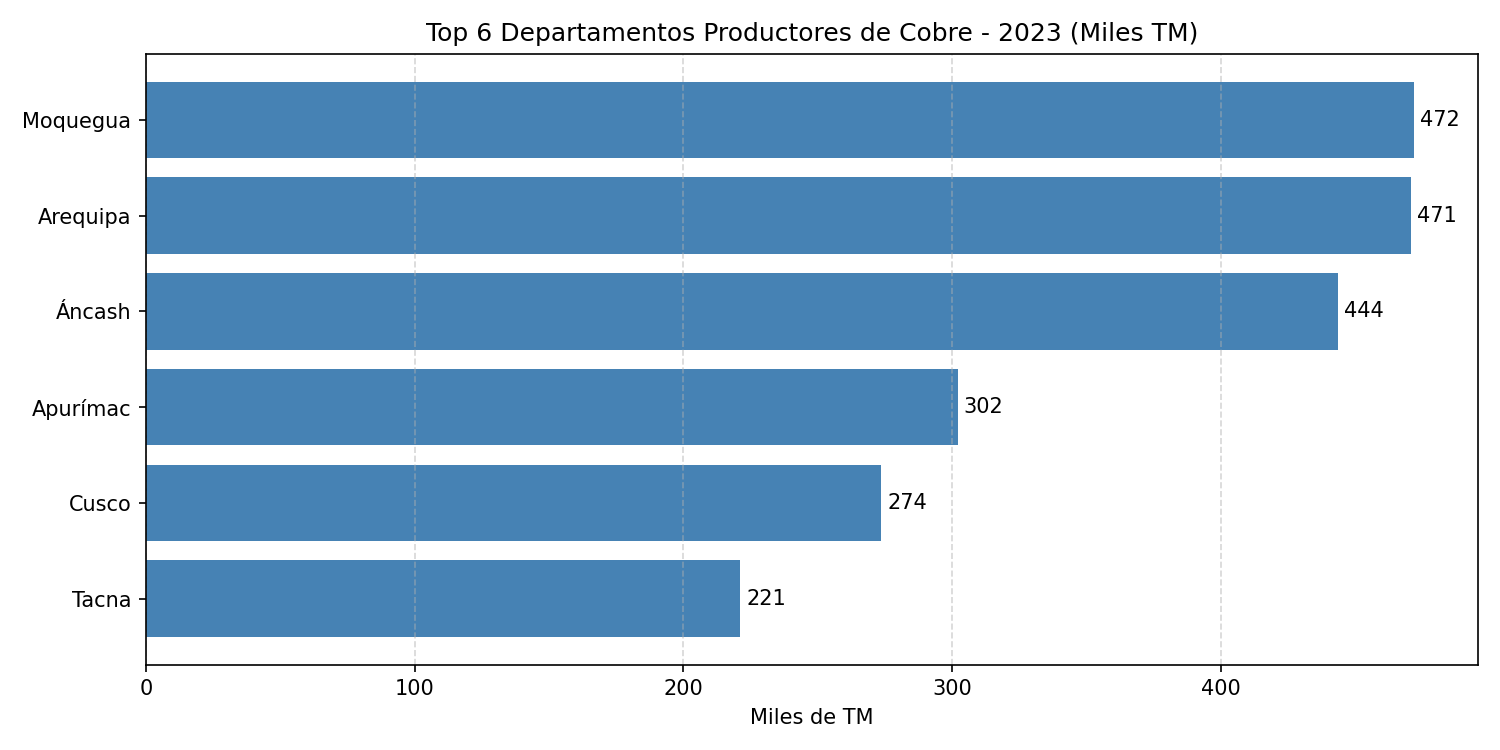
\includegraphics[width=0.9\textwidth]{grafico_14_5b.png}
\caption{Top 6 departamentos productores de cobre -- 2023}
\end{figure}

\subsection{Producción de plata}

\begin{figure}[H]
\centering
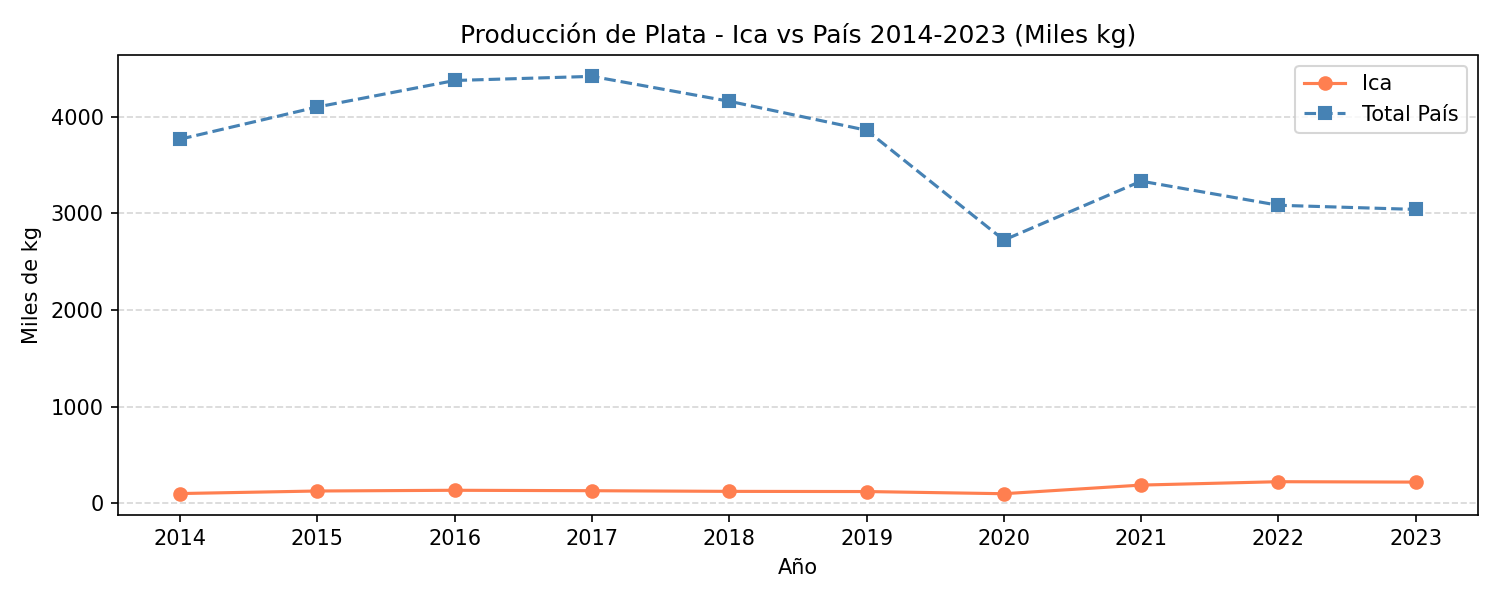
\includegraphics[width=0.9\textwidth]{grafico_14_6a.png}
\caption{Producción de plata -- Ica vs País, 2014--2023 (Miles kg)}
\end{figure}

\begin{figure}[H]
\centering
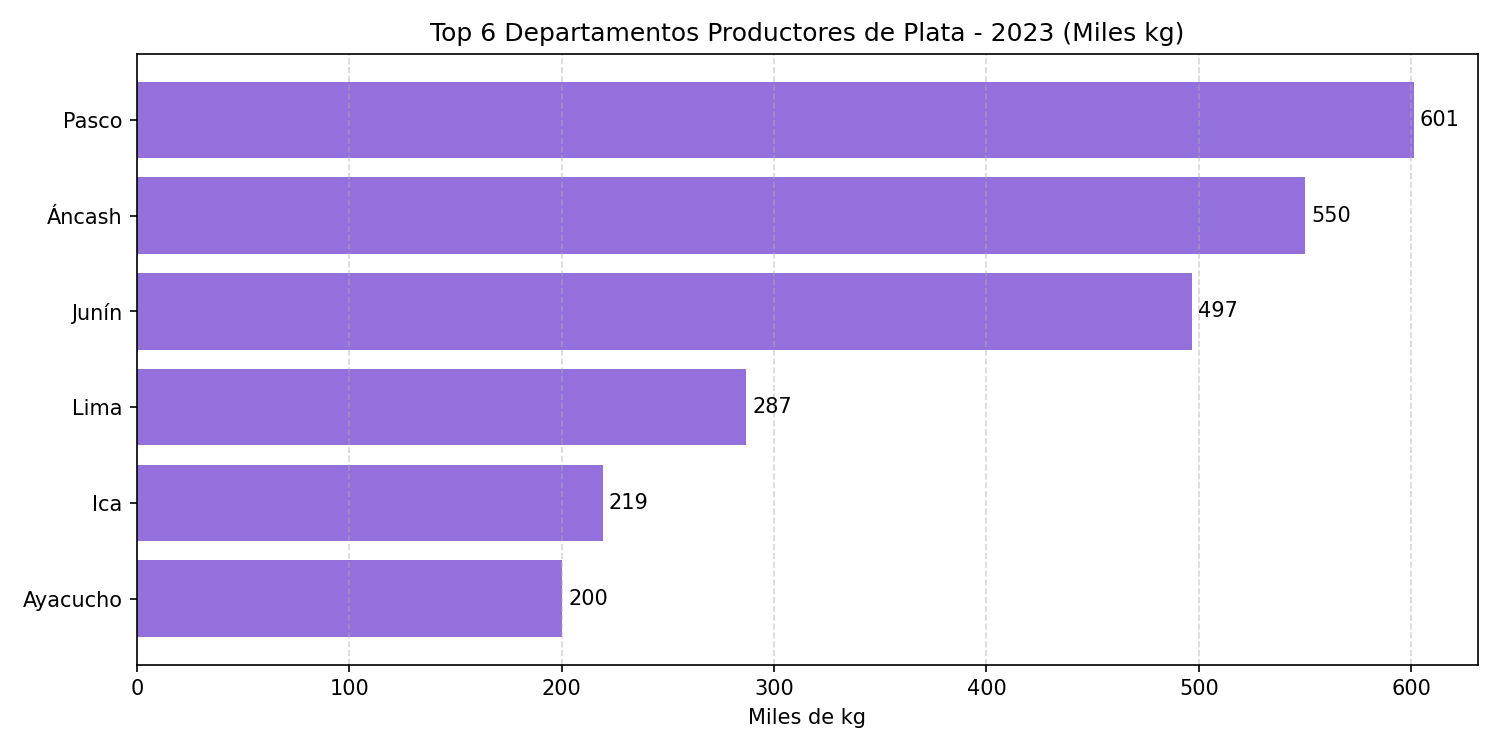
\includegraphics[width=0.9\textwidth]{grafico_14_6b.png}
\caption{Top 6 departamentos productores de plata -- 2023}
\end{figure}

\subsection{Exportación minera nacional}

\begin{table}[H]
\centering
\caption{Valor Exportación FOB Minera - Perú, 2014-2023 (Mill. US\$)}
\small
\begin{tabular}{lrrrrr}
\toprule
\textbf{Año} & \textbf{Total} & \textbf{Cobre} & \textbf{Oro} & \textbf{Zinc} & \textbf{Plomo} \\
\midrule
2,014.00 & 20,545.41 & 8,874.91 & 6,729.07 & 1,503.55 & 1,522.51 \\
2,015.00 & 18,950.14 & 8,167.54 & 6,650.60 & 1,507.66 & 1,548.27 \\
2,016.00 & 21,819.08 & 10,170.88 & 7,425.71 & 1,468.76 & 1,657.81 \\
2,017.00 & 27,581.61 & 13,844.96 & 8,270.48 & 2,398.51 & 1,726.13 \\
2,018.00 & 28,898.66 & 14,938.55 & 8,258.51 & 2,573.90 & 1,545.47 \\
2,019.00 & 28,336.21 & 14,000.93 & 8,555.12 & 2,114.02 & 1,566.97 \\
2,020.00 & 26,127.69 & 13,039.53 & 7,829.57 & 1,707.15 & 1,460.63 \\
2,021.00 & 39,900.75 & 20,694.20 & 10,184.99 & 2,685.08 & 2,028.33 \\
2,022.00 & 38,105.89 & 19,671.80 & 10,194.40 & 2,677.08 & 1,786.32 \\
2,023.00 & 42,789.55 & 23,429.05 & 10,942.70 & 2,356.11 & 1,919.80 \\
\bottomrule
\end{tabular}
\end{table}


\begin{figure}[H]
\centering
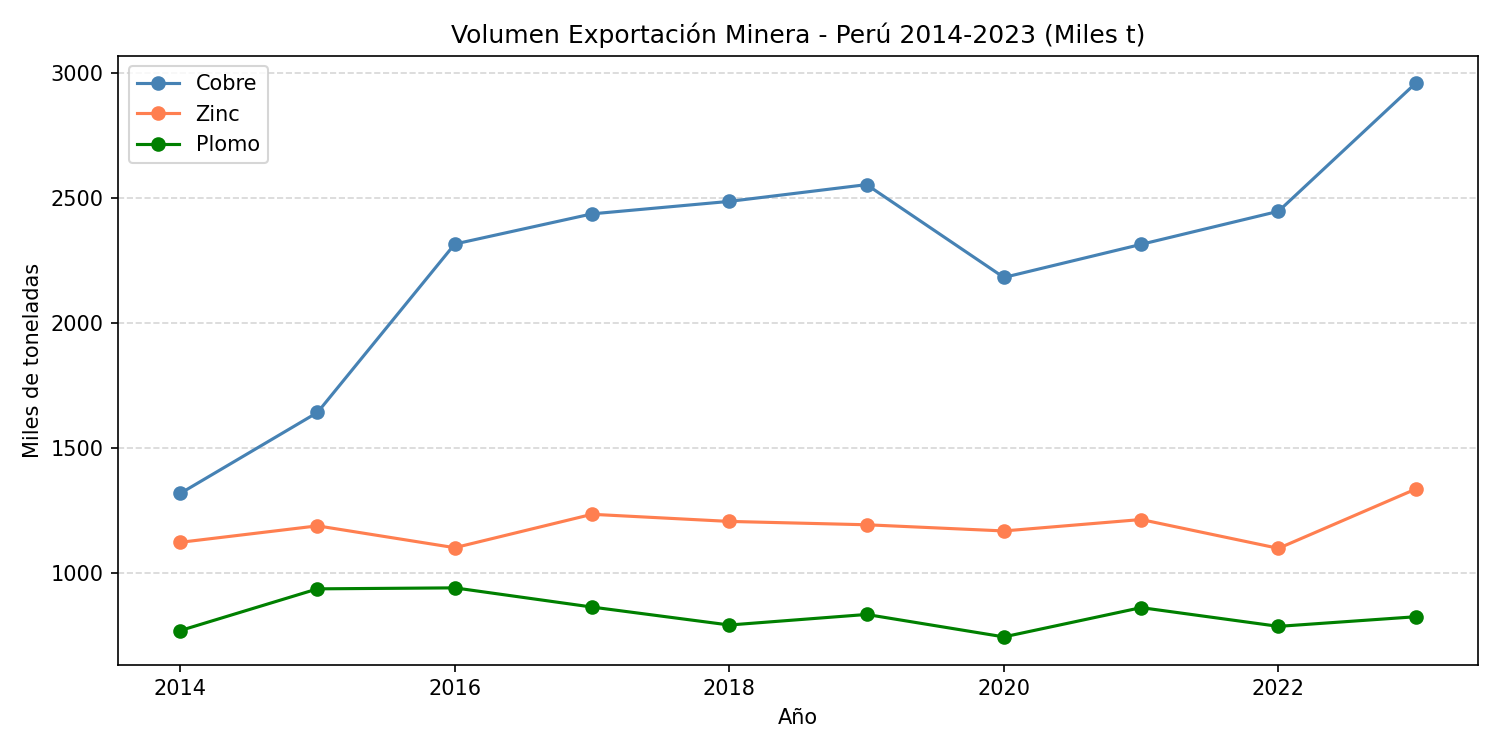
\includegraphics[width=0.9\textwidth]{grafico_14_11a.png}
\caption{Volumen exportación minera -- Perú, 2014--2023 (Miles TM)}
\end{figure}

\begin{figure}[H]
\centering
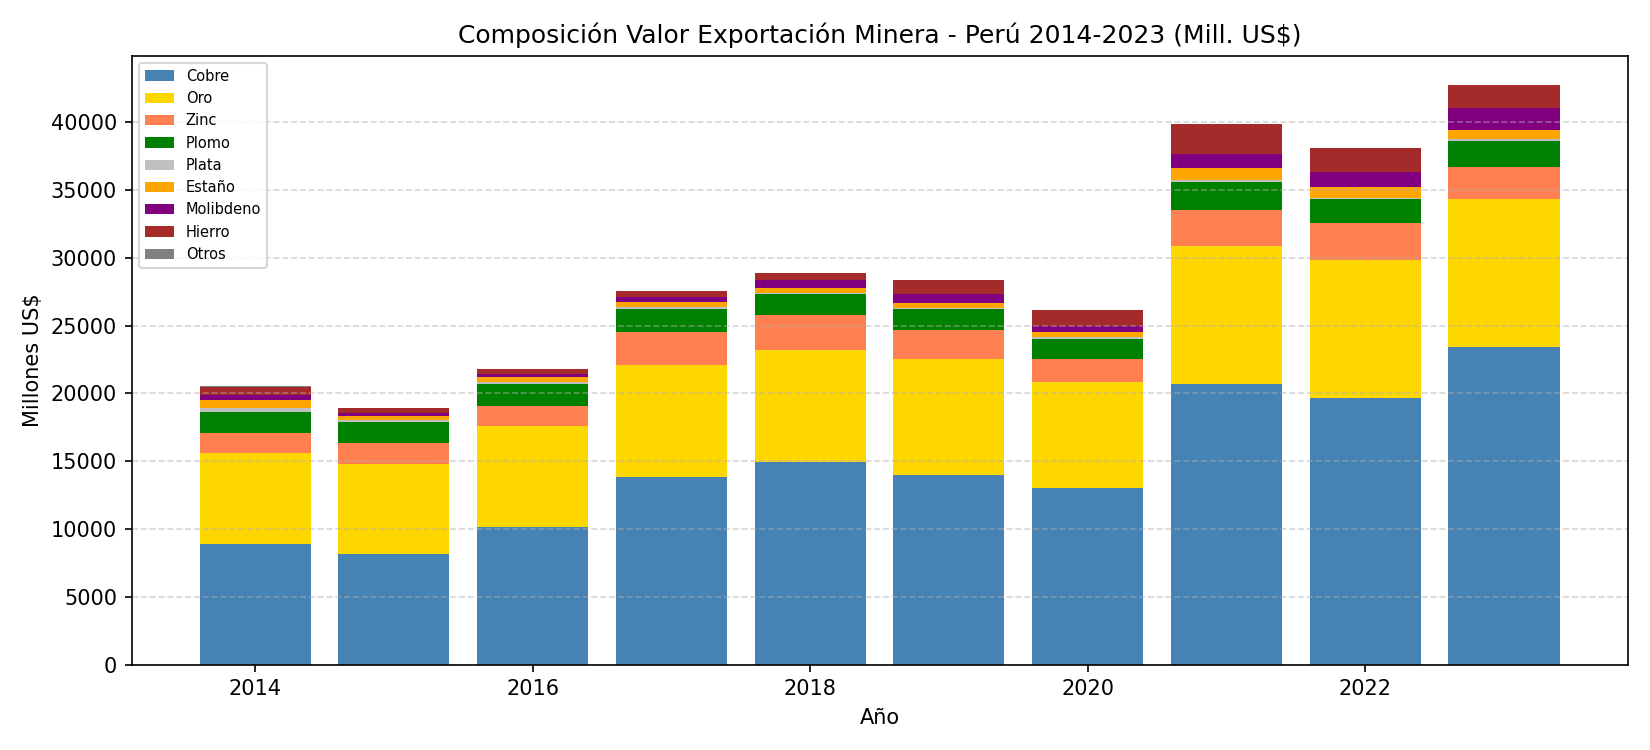
\includegraphics[width=0.9\textwidth]{grafico_14_12b.png}
\caption{Composición valor exportación minera FOB -- Perú, 2014--2023}
\end{figure}

\subsection{Interpretación}
El crecimiento de la minería en Ica durante el período analizado es
destacable. La producción de cobre pasó de 43,155 TM en 2016 a
216,349 TM en 2023, un incremento de casi cinco veces en siete años.
Este crecimiento posicionó a Ica entre los principales productores
de cobre del país, siendo superado solo por departamentos con mayor
tradición minera como Áncash y Arequipa.

El zinc es el mineral de mayor volumen en Ica, aunque con una tendencia
más estable. La plata también muestra un crecimiento importante desde
2020, pasando de 98,945 kg a 219,199 kg en 2022. A nivel nacional,
el cobre y el oro dominan el valor de las exportaciones mineras,
con el cobre representando más del 50\% del total en 2023.

%---------------------------------------
\section{Sector 15: Manufactura}
%---------------------------------------
\subsection{Descripción del indicador}
El indicador 15.9 registra la producción de conservas y empacado de
frutas, hortalizas, legumbres y derivados en Ica, expresada en
toneladas, para el período 2011--2020.

\subsection{Análisis descriptivo}

\begin{figure}[H]
\centering
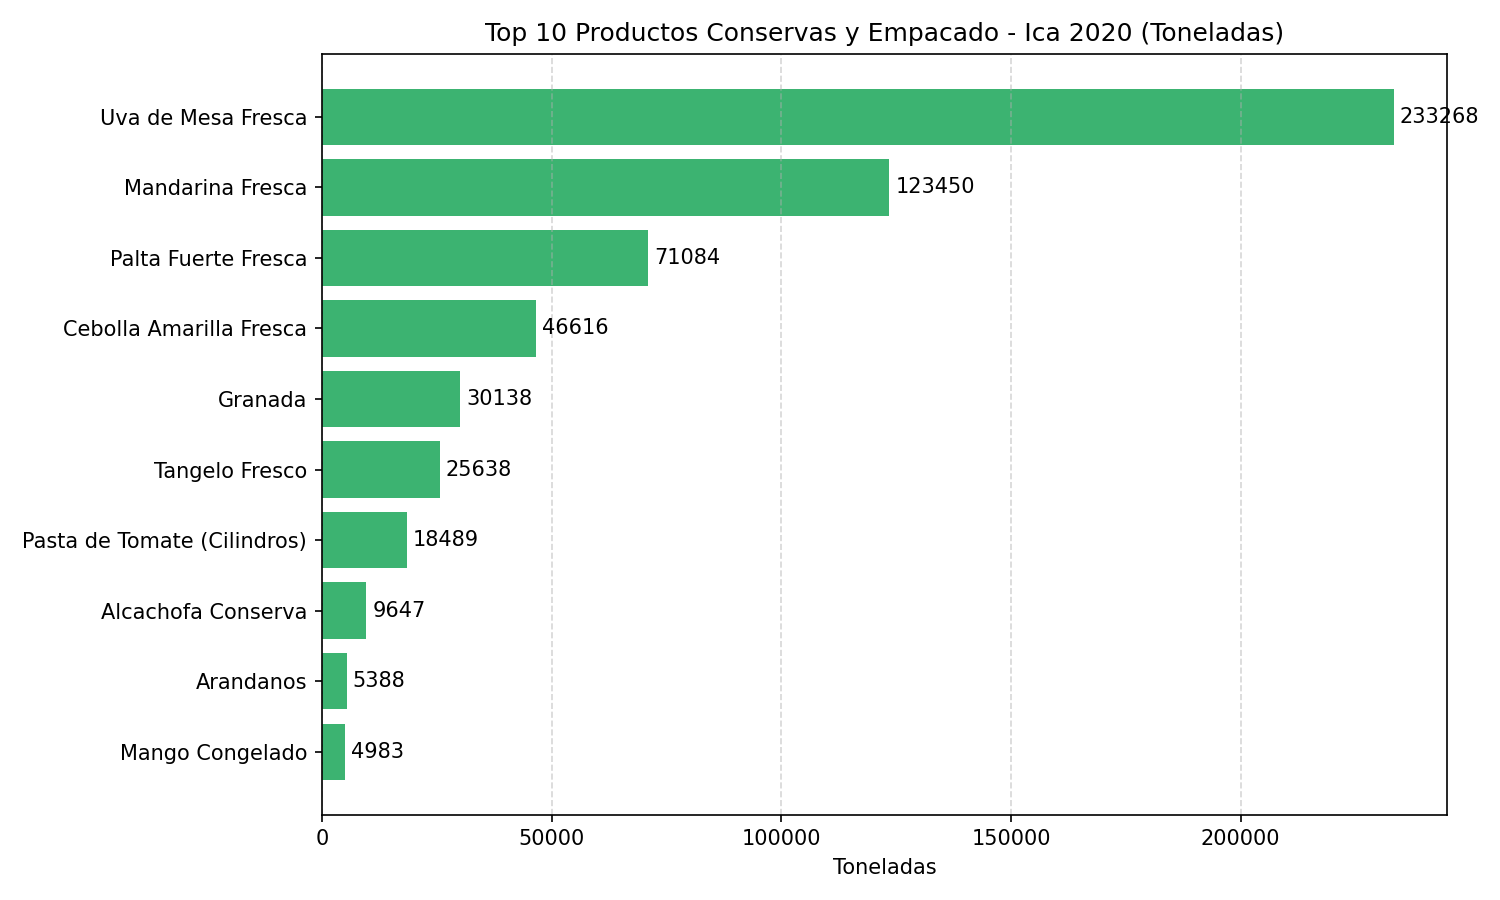
\includegraphics[width=0.9\textwidth]{grafico_15_9a.png}
\caption{Top 10 productos de conservas y empacado -- Ica, 2020 (TM)}
\end{figure}

\begin{figure}[H]
\centering
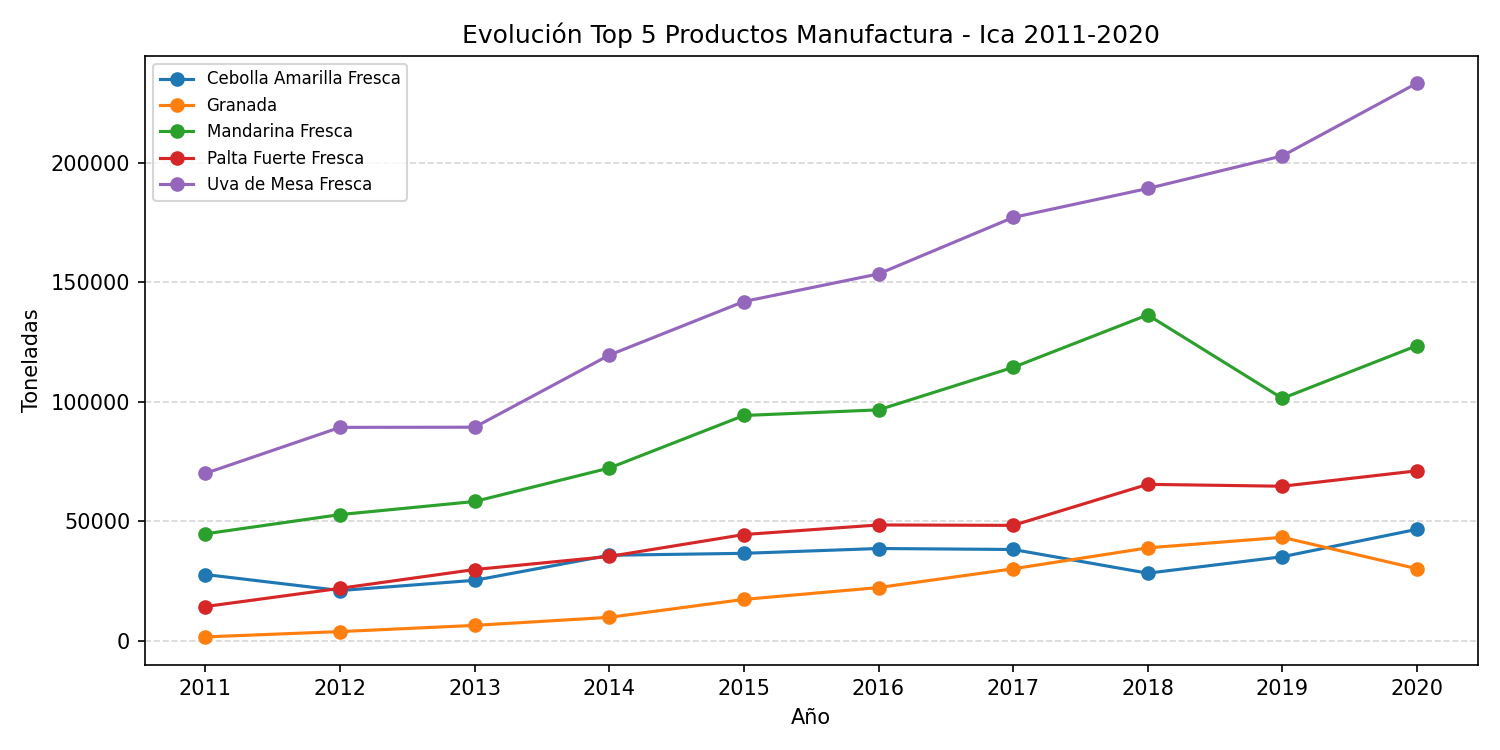
\includegraphics[width=0.9\textwidth]{grafico_15_9b.png}
\caption{Evolución top 5 productos manufactura -- Ica, 2011--2020}
\end{figure}

\subsection{Interpretación}
La manufactura de conservas y empacado en Ica refleja directamente
la estructura productiva agrícola de la región. La mandarina fresca
lidera la producción con 123,450 TM en 2020, seguida de la uva y
el espárrago. Resulta llamativa la evolución de la granada, que pasó
de 1,603 TM en 2011 a 30,138 TM en 2020, lo que evidencia la
diversificación de la canasta agroexportadora iqueña hacia cultivos
de mayor valor en el mercado internacional.

%---------------------------------------
\section{Sector 16: Electricidad y Agua}
%---------------------------------------
\subsection{Descripción del indicador}
El indicador 16.1 recoge la potencia de energía eléctrica instalada
en Ica, clasificada por tipo de servicio (público y privado) y por
fuente de generación (hidráulica, térmica y eólica), expresada en
megavatios (MW), para el período 2006--2022.

\subsection{Análisis descriptivo}

\begin{figure}[H]
\centering
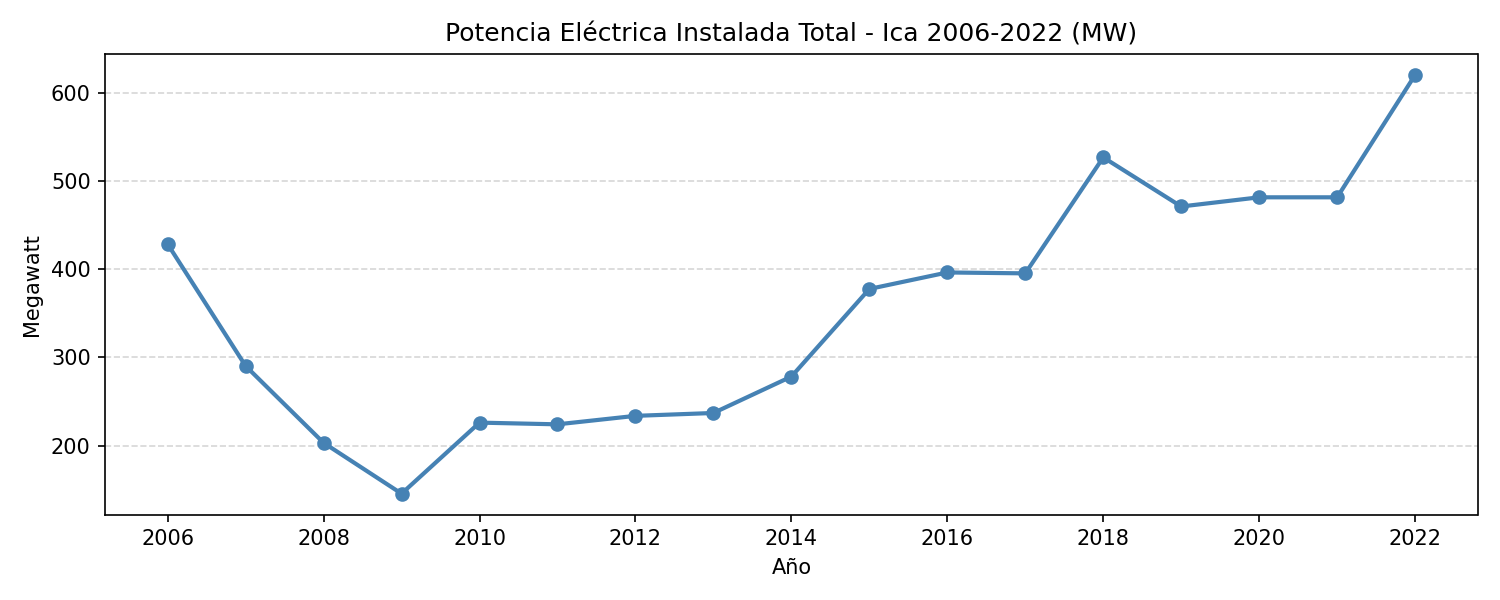
\includegraphics[width=0.9\textwidth]{grafico_16_1a.png}
\caption{Potencia eléctrica instalada total -- Ica, 2006--2022 (MW)}
\end{figure}

\begin{figure}[H]
\centering
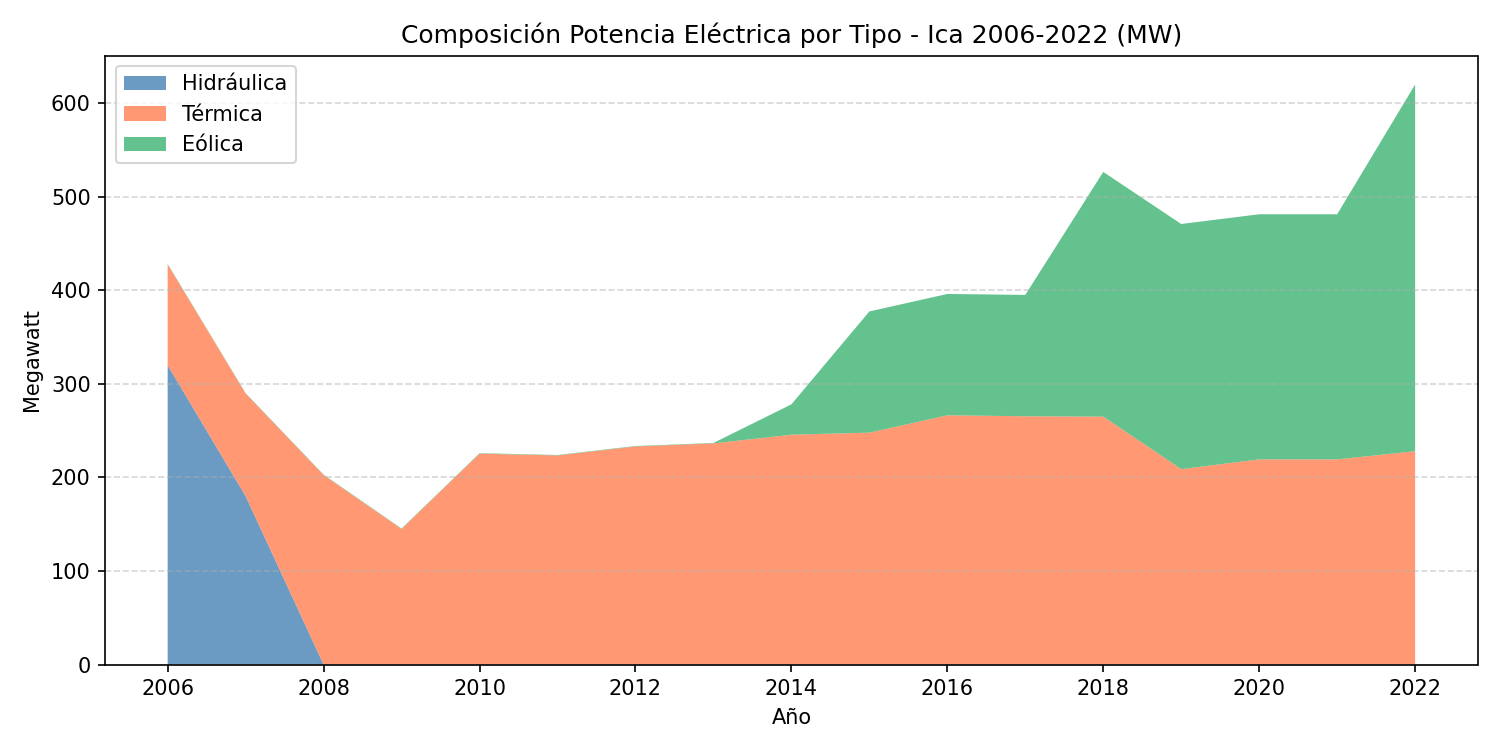
\includegraphics[width=0.9\textwidth]{grafico_16_1b.png}
\caption{Composición de la potencia eléctrica por tipo -- Ica, 2006--2022}
\end{figure}

\subsection{Interpretación}
La capacidad eléctrica instalada en Ica creció de 428 MW en 2006
a 620 MW en 2022, lo que representa un incremento del 44.9\% en
16 años. El cambio más significativo en la composición de la matriz
energética iqueña fue la incorporación de la energía eólica a partir
de 2015, con una potencia instalada de 129.6 MW que se mantuvo
estable hasta 2022, cuando se amplió a 392 MW. Esta diversificación
responde a la política nacional de promoción de energías renovables
y a las condiciones de viento favorables en la costa de Ica.

La generación hidráulica, que era relevante en 2006 y 2007,
desapareció desde 2008, siendo reemplazada completamente por
fuentes térmicas y posteriormente eólicas.

%---------------------------------------
\section{Sector 17: Construcción}
%---------------------------------------
\subsection{Descripción del indicador}
El indicador 17.1 presenta los principales indicadores del sector
construcción a nivel nacional, incluyendo el PBI global, el Valor
Agregado Bruto (VAB) del sector, la variación porcentual anual y
los indicadores del mercado de cemento, para el período 2016--2023.

\subsection{Análisis descriptivo}

\begin{table}[H]
\centering
\caption{Indicadores Sector Construcción - Perú, 2016-2023}
\small
\begin{tabular}{lrrrrrrrr}
\toprule
\textbf{Indicador} & \textbf{2016} & \textbf{2017} & \textbf{2018} & \textbf{2019} & \textbf{2020} & \textbf{2021} & \textbf{2022} & \textbf{2023} \\
\midrule
PBI global (Millones S/) & 647,668.00 & 687,989.00 & 731,588.00 & 761,984.00 & 703,914.96 & 878,380.49 & 945,329.29 & 1,001,860.48 \\
VAB (Millones S/) & 42,610.00 & 45,134.00 & 49,648.00 & 51,148.00 & 47,571.31 & 66,416.70 & 72,715.00 & 73,043.00 \\
Variación % anual & -2.64 & 2.43 & 5.41 & 1.46 & -14.91 & 34.89 & 2.58 & -7.95 \\
\bottomrule
\end{tabular}
\end{table}


\begin{figure}[H]
\centering
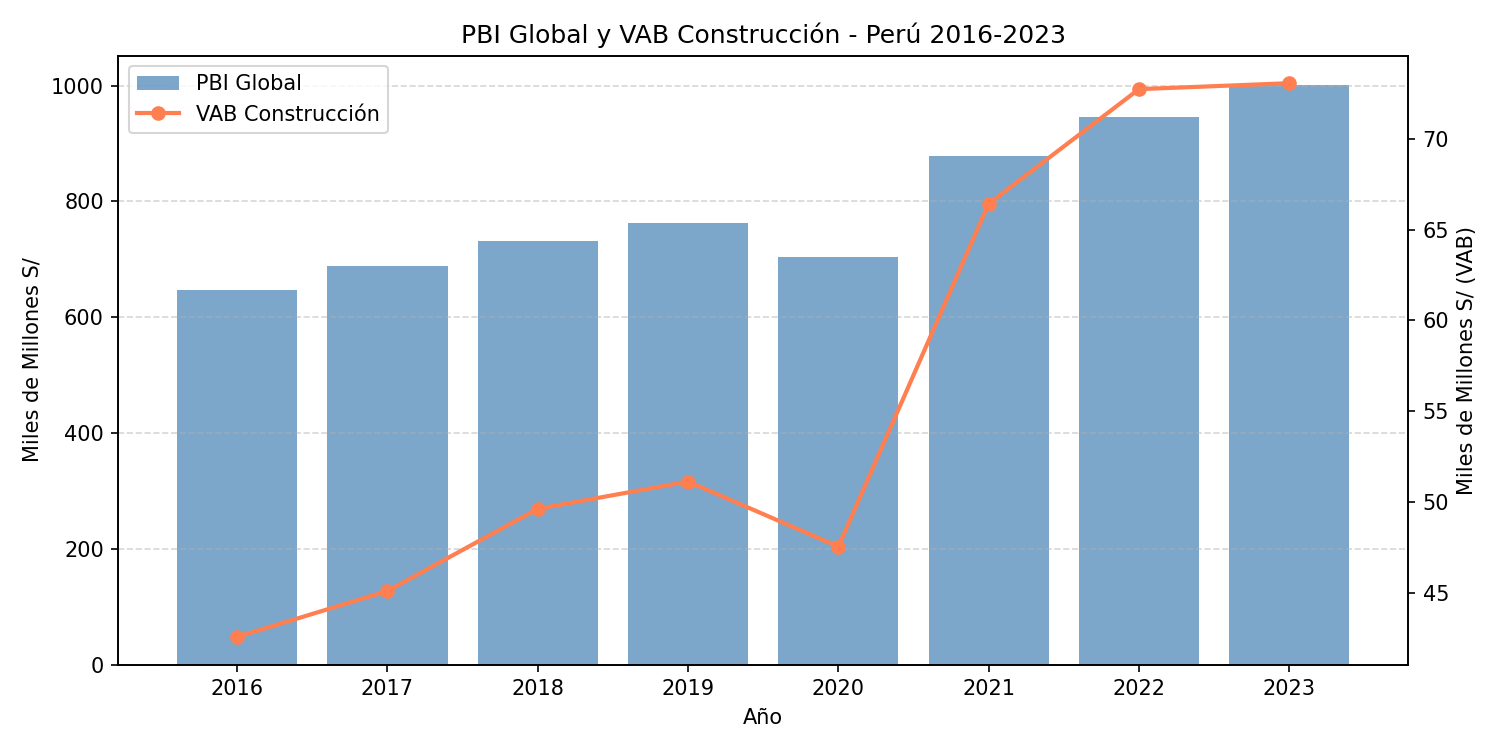
\includegraphics[width=0.9\textwidth]{grafico_17_1a.png}
\caption{PBI global y VAB construcción -- Perú, 2016--2023}
\end{figure}

\begin{figure}[H]
\centering
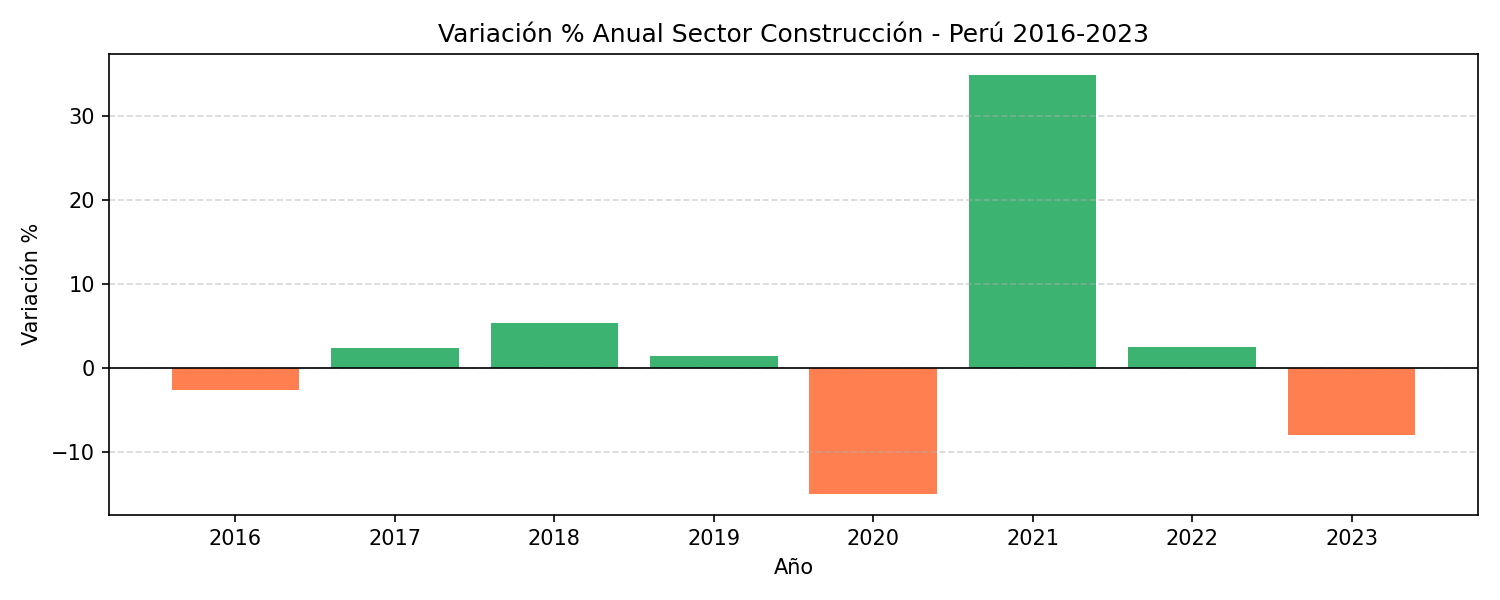
\includegraphics[width=0.9\textwidth]{grafico_17_1b.png}
\caption{Variación \% anual sector construcción -- Perú, 2016--2023}
\end{figure}

\begin{figure}[H]
\centering
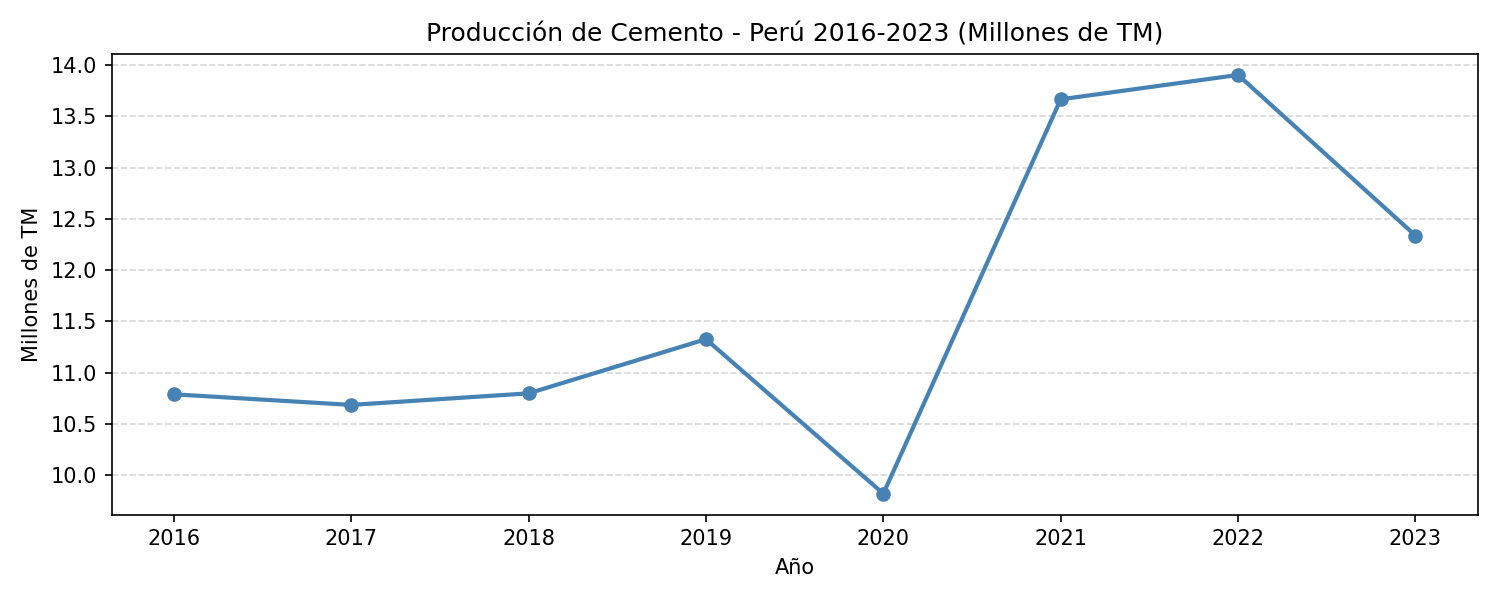
\includegraphics[width=0.9\textwidth]{grafico_17_1c.png}
\caption{Producción de cemento -- Perú, 2016--2023 (Millones TM)}
\end{figure}

\subsection{Interpretación}
El sector construcción mostró un comportamiento volátil durante
el período analizado. Tras años de crecimiento moderado entre 2016
y 2019, registró una caída histórica de 14.91\% en 2020 como
consecuencia directa de las medidas de confinamiento por la pandemia.
La recuperación en 2021 fue igualmente extraordinaria, con un
crecimiento de 34.89\%, impulsado por la reactivación de obras
públicas y privadas postergadas.

Sin embargo, en 2023 el sector volvió a contraerse en 7.95\%,
lo que podría estar relacionado con la reducción del gasto público
en infraestructura y la menor inversión privada en un contexto
de incertidumbre política. La producción de cemento sigue una
tendencia similar, con un pico en 2021 de 13.7 millones de TM
y una caída posterior en 2023.

%---------------------------------------
\section{Conclusiones}
%---------------------------------------
A partir del análisis de los ocho sectores estudiados, se pueden
extraer las siguientes conclusiones sobre la dinámica socioeconómica
del departamento de Ica:

\begin{itemize}
    \item La documentación de identidad en Ica se mantiene en niveles
    muy altos, aunque la pandemia generó una caída temporal que se
    revirtió en 2023.

    \item En el ámbito TIC, la región experimenta una transición clara
    desde tecnologías tradicionales como el teléfono fijo y la radio
    hacia dispositivos móviles y plataformas digitales.

    \item El sector agrario es el más dinámico de la economía iqueña,
    con la uva, la mandarina y la palta liderando el crecimiento
    de la producción y las exportaciones.

    \item La actividad pesquera muestra una recuperación sostenida
    desde 2016, con Pisco como principal centro de desembarque.

    \item La minería, especialmente la producción de cobre, ha
    experimentado un crecimiento excepcional en Ica, consolidándose
    como un sector estratégico para la región.

    \item La manufactura de conservas refleja la fortaleza
    agroexportadora de Ica, con una canasta de productos cada vez
    más diversificada.

    \item La matriz energética de Ica se ha modernizado con la
    incorporación de energía eólica, reduciendo la dependencia
    de fuentes térmicas.

    \item El sector construcción, tanto a nivel nacional como
    regional, sigue siendo sensible a los ciclos económicos y
    a las decisiones de política pública en materia de inversión.
\end{itemize}

\end{document}
